\documentclass[aspectratio=169]{beamer}
\usepackage[utf8]{inputenc}
\usepackage{tikz}
\usetikzlibrary{arrows.meta, positioning}
\setbeamertemplate{bibliography item}{\insertbiblabel}
\usepackage{multirow,rotating}
\usepackage{color}
\usepackage{hyperref}
\usepackage{tikz-cd}
\usepackage{array}
\usepackage{ragged2e}
\usepackage{siunitx}
\usepackage{mathtools,nccmath}%
\usepackage{amsmath}
\usepackage{caption}
\usetikzlibrary{decorations.pathreplacing}  %  for the timeline
\usepackage{booktabs}
\usepackage{threeparttable}   % table notes under the tabular
\usepackage{siunitx}          % numeric alignment (preferred over dcolumn)
\sisetup{
  detect-mode,
  detect-family, detect-inline-family=math,
  input-symbols = {()}, table-align-text-post=false,
  group-separator = {,}, group-minimum-digits = 4
}
\usepackage{adjustbox}        % optional: fit table to width
\usepackage[labelsep=period]{caption}

\usepackage{etoolbox, xparse}
\usepackage[dvipsnames]{xcolor}
\usepackage{threeparttable}

\usepackage{soul}
\makeatletter
\let\HL\hl
\renewcommand\hl{%
  \let\set@color\beamerorig@set@color
  \let\reset@color\beamerorig@reset@color
  \HL}
\makeatother
\usetheme{CambridgeUS}
\usecolortheme{dolphin}
\setbeamertemplate{headline}{} %eliminates the red line above with the section
\setbeamertemplate{navigation symbols}{}

%%% to adjust the footline
\setbeamertemplate{footline}{%
  \leavevmode%
  \hbox{%
    \begin{beamercolorbox}[wd=\paperwidth,ht=3.5ex,dp=2ex,
        leftskip=1em,rightskip=1em]{author in head/foot}%
      \usebeamerfont{author in head/foot}%
      \insertshortauthor \hfill \insertshorttitle \hfill \insertframenumber/\inserttotalframenumber
    \end{beamercolorbox}%
  }%
}
\usetikzlibrary{arrows.meta,
                chains,
                positioning,
                shapes.geometric
                }
\usepackage{tikz}
\usepackage{setspace}

% set colors
\definecolor{myNewColorA}{RGB}{158, 27,50}
\definecolor{myNewColorB}{RGB}{158, 27,50}
\definecolor{myNewColorC}{RGB}{158, 27,50} % {130,138,143}
\setbeamercolor*{palette primary}{bg=myNewColorC}
\setbeamercolor*{palette secondary}{bg=myNewColorB, fg = white}
\setbeamercolor*{palette tertiary}{bg=myNewColorA, fg = white}
\setbeamercolor*{titlelike}{fg=myNewColorA}
\setbeamercolor*{title}{bg=myNewColorA, fg = white}
\setbeamercolor*{item}{fg=myNewColorA}
\setbeamercolor*{caption name}{fg=myNewColorA}
\usefonttheme{professionalfonts}
\usepackage{natbib}
\usepackage{hyperref}


% Redefinir el comando \beamergotobutton
\setbeamercolor{button}{bg=gray,fg=white} % Fondo gris y texto blanco
\setlength{\parskip}{0.9em}  % aumentar el espacio entre parrafos

% To show only the number of specific slides

\usepackage{appendixnumberbeamer}

%------------------------------------------------------------

%------------------------------------------------------------
% \titlegraphic{\includegraphics[height=0.75cm]{ua_eng_logo.png}}
% logo of my university

\setbeamerfont{title}{size=\large}
\setbeamerfont{subtitle}{size=\small}
\setbeamerfont{author}{size=\small}
\setbeamerfont{date}{size=\footnotesize}
\setbeamerfont{institute}{size=\footnotesize}

\title[The Political Legacy of Displacement]{The Political Legacy of Displacement:}
\subtitle{\large Evidence from the Spanish Exile}

\author[Aranzana, C. \& Paluskiewicz, L.]{Cristina Aranzana$^{*}$ \& Luc Paluskiewicz$^{\dagger}$\\
\vspace{0.25cm}
\scriptsize $^{*}$University of Barcelona \& IEB \\
\scriptsize $^{\dagger}$Paris School of Economics
}


\date{March 2026}

\begin{document}


% Title slide (not counted)
\begingroup
  \setbeamertemplate{footline}{} % remove footline for title
  \begin{frame}[plain]
    \titlepage

    % Logos in bottom corners
    \begin{tikzpicture}[remember picture,overlay]
      \node[anchor=south west, xshift=0.5cm, yshift=0.5cm]
        at (current page.south west)
        {
\includegraphics[height=0.8cm]{pictures/logo_ub}};
      \node[anchor=south east, xshift=-0.5cm, yshift=0.5cm]
        at (current page.south east)
        {
\includegraphics[height=1cm]{pictures/logo_ieb}};
    \end{tikzpicture}

  \end{frame}
\endgroup

\setcounter{framenumber}{0}

%------------------------------------------------------------


\begin{frame}{Motivation}

\begin{itemize}

  \item 117.3 million people had been forced to flee their homes globally (UNHCR, 2025).
  \item Politically motivated persecution generates ideological selection into exile.
  \item Receiving societies exhibit a sustained rise in anti-immigrant attitudes (IOM, 2024)
% Studying how host political backlash emerges, propagates, and persists matters for understanding the long-run political consequences of forced migration.
\vspace{0.4cm}
  \item \textbf{How do politically selected refugees shape voting and collective action in host communities?}
\begin{itemize}
\item We study the political consequences of the 1939 mass displacement of Spanish Republicans into France ("La Retirada").
%republcians here refer to left-wing
%Temporary, forced contact with foreigners. Even though it was a culturally similar and mostly educated refugee shock, it trigger a negative reaction.
\end{itemize}
\end{itemize}

%https://worldmigrationreport.iom.int/what-we-do/world-migration-report-2024-chapter-1/what-has-happened-migration

%Unlike economic migrants driven chiefly by jobs, refugees are often politically selected – meaning they represent a specific ideological or demographic subset of their home country.

%As of the end of June 2025, the most recent reporting period, 117.3 million people had been forced to flee their homes globally due to persecution, conflict, violence, human rights violations or events seriously disturbing public order.
%1 in every 70 people on Earth has been forced to flee

% https://www.unhcr.org/about-unhcr/overview/figures-glance
%Becker and Ferrara (2019) argue that forced migration can have distinct consequences for the migrants themselves because of the forceful nature of the displacement experience as well the loss of possessions and homes against their own will. While voluntary migration is likely to follow economic cost–benefit considerations of the migrants, involuntary migration is the result of forces that are largely outside the control of the migrants.
%Fourth, the long-term consequences of forced displacement permit a unique perspective not only on how forced migration happened but also on the legacy of forced displacement on populations at destination and origin,
%A promising area with so far little research is that of selective migration in the face of persecution. While there are many cases of (near-)universal expulsion that have been studied, there are episodes where despite persecution not all those targeted by it do emigrate.

\end{frame}

%\begin{frame}{Preview}

%\begin{itemize}

%  \item \textbf{Research Question:} how do politically selected refugees shape political outcomes in host communities?
%\vspace{0.4cm}
%\begin{itemize}
%  \item We study the 1939 mass displacement of Spanish Republicans into France ("La Retirada") to estimate the effects on voting and collective action.
%\end{itemize}
%\vspace{0.4cm}
%  \item We employ a two-way fixed-effects estimator that accounts for spatial spillovers using concentric circles.
%  \item \textbf{Preliminary Results:} communes exposed to refugee camps display lower support for the socialist party. Suggestive evidence indicates that the type of contact matters.

%\end{itemize}


%\end{frame}

\section{Contribution}

\begin{frame}{Contribution}




\begin{itemize}
    \item Our research contributes to several strands of literature:
    \begin{itemize}
        \item The effect of refugee exposure on political outcomes \textcolor{gray}{\citep{halla_immigration_2017, dustmann_refugee_2018,hangartner_refugee_2019, edo_immigration_2019, steinmayr_contact_2021, alesina_political_2024}}. %
        \item The impact of historical immigration shocks at the destination country in the long-run \textcolor{gray}{\citep{tabellini_gifts_2020, schindler_shocking_2021,bursztyn_immigrant_2024, chevalier_forced_2024, ochsner_activated_2024, toews_enemies_2025}}. %
        \item The effect of migration on the diffusion of political ideas \textcolor{gray}{\citep{spilimbergo_democracy_2009, barsbai_effect_2017,dippel_leadership_2021, calderon_racial_2023, bazzi_confederate_2023}}   %
        %dippel and Heblich, 2021: leaders of the failed german revolution of 1848 (forty-eighters) contribute to the social movement against slavery.
    \end{itemize}
\end{itemize}

%We differentiate ourselves because we are not talking about the effect of leaders, as the leaders of the central government, catalan and basque were not in concentration camps.

%El presidente de la República, Manuel Azaña, cruzó la frontera y falleció ese mismo año en Montauban (sur de Francia)
%Juan Negrin (ultimo jefe del gobierno republicano) se exilió a Reino Unido (aunque murió en Paris)
%Jose Antonio Aguirre: estableciendo en Nueva York una delegación vasca aliada con los servicios británicos y norteamericanos durante la Segunda Guerra Mundia. José Antonio Aguirre y Lecube, en euskera, Jose Antonio Agirre Lekube (Bilbao, Vizcaya, 6 de marzo de 1904-París, 22 de marzo de 1960) fue un político español, militante del Partido Nacionalista Vasco
%Indalecio Prieto: Mexico fue un político español del Partido Socialista Obrero Español (PSOE), titular de las carteras ministeriales de Hacienda, Obras Públicas, Marina y Aire y Defensa Nacional durante la Segunda República. Exiliado en México tras la derrota republicana en la guerra civil española, desempeñó la presidencia del PSOE entre 1948 y 1951.
%Pompeu Fabra: Prada de Conflent
%Josep Tarradellas: fue un político español, presidente de la Generalidad de Cataluña en el exilio desde 1954 hasta 1977, y de la Generalidad provisional desde esta fecha hasta 1980.Saint Martin-Le-Beau
%Federica Montseny: Toulouse sindicalista



\end{frame}


\begin{frame}[label=Hypothesis]{Hypothesis}


%The effect is theoretical ambiguos

\begin{itemize}
    \item \textbf{Political diffusion \& participation:} contact between the local population and the refugees can reduce prejudice (Allport, 1954) but also foster diffusion of ideas. \hyperlink{Presse2}{\beamergotobutton{Example}}
    \vspace{0.4cm}
    \item \textbf{Native backlash:} the ideas that the refugees bring may be perceived as a threat, reducing the support of the values they represent. \hyperlink{Presse1}{\beamergotobutton{Example}}
\end{itemize}

\end{frame}


%15259 adquired the french nationality. Moreover, newly naturalized individuals remained subject to legal incapacities: they were excluded from the electoral rolls for five years after naturalization and barred from holding elected office for ten years \citep{code_nationalite_fr_1945}. For these reasons, the settlement of Spanish refugees could not have mechanically translated into direct electoral participation.


\section{Historical context}

\begin{frame}{La Retirada}

%The Spanish Civil War began in 1936 with Francisco Franco's military coup against the Second Spanish Republic, confronting Franco's forces with various left-wing groups – republicans, anarchists, communists. As the war progressed, by 1939 Catalonia was one of the last places under Republican control.

%The Basque Country had fallen. Only Madrid and the east resisted, so there has been also important internal displacement of poeple.  By then the Republic's situation was desperate.

%A bit more than 50% are going to be from Catalunia and Aragon.
%East (14%)
%Andalucia (10%)
%the other 25% the rest

  \begin{itemize}
% With the onset of the Spanish Civil War in 1936 and the advance of Franco's troops many republicans found refugee in Catalonia.
  \item The defeat of the republican forces in Barcelona in January 1939 precipitated a mass exodus of close to \textbf{half a million people} towards France knowns as ``The Retirada".
  \item Spanish refugees were interned in camps for the following months, forced to remain where assigned.
\end{itemize}
%Considering the last census available of 1936, the total population of France was 41967056 habitants, this represents 1,19% of the population. The shock represents 22% of the total foreign population in 1939. The total foreign population was 2198236 in 1939.
  \begin{center}
    
\includegraphics[width=0.4\textwidth]{pictures/image2.jpg}
  \end{center}

\end{frame}

\begin{frame}{Dispersion policy}

  \begin{itemize}
  \item Men of military age were mostly held in camps near the border, while the civilian population was transferred to reception centers dispersed across France.
  \item Because no permanent facilities had been prepared in advance, the selection of camp sites was rushed and chaotic.
\end{itemize}

  \begin{center}
    
\includegraphics[width=0.6\textwidth]{pictures/Retirada.jpg}
  \end{center}
\end{frame}

\begin{frame}{Context in France}

  \begin{itemize}
%under the surveillance of the authorities
  \item French authorities encouraged return to Spain or emigration to third countries.
  % the CIARE calculated that around 400,000 people had crossed into France. Of these, 60,000 had already returned to the peninsula by July 1939. By the end of 1939, the number of exiles in France was 140000 (more political selection). Some countries in Latinoamerica welcomed refugees.
  % they  promote ``voluntary" return through incentives and coercion. By early August, around 250,000 refugees had returned to Spain
  \item  Those who stayed were sent to labour brigades, the Foreign Legion, and 15.000 joined the Resistance.
  %By late 1939, an estimated 50,000–60,000 Spaniards were serving in these militarized work companies across France and 7000 join the Foreign Legion \citep{academicoup} % EXPLAIN HERE THE OCCUPATION. Thousands of Spanish Republicans were subsequently deported to Nazi concentration camps—most notoriously Mauthausen, where approximately 7,000 died.
  \item By the end of WWII, 160.000 remained in France.
\end{itemize}


\centering
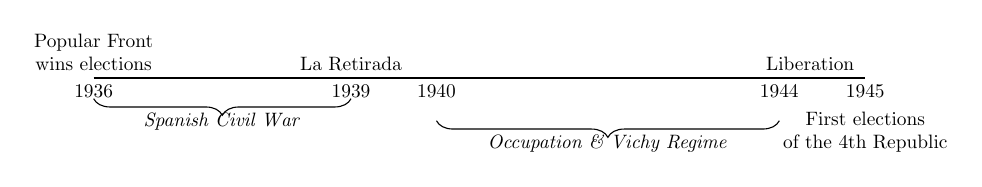
\begin{tikzpicture}[scale=0.7, transform shape]

\draw[thick] (0,0) -- (14,0);

\node[below] at (0,0) {1936};
\node[below] at (4.67,0) {1939};
\node[below] at (6.22,0) {1940};
\node[below] at (12.44,0) {1944};
\node[below] at (14,0) {1945};

\node[above, align=center] at (0,0) {Popular Front \\ wins elections};

\draw[decorate, decoration={brace, amplitude=6pt}, yshift=-8pt]
  (4.67,-0.1) -- (0,-0.1)
  node[midway, yshift=-12pt] {\textit{Spanish Civil War}};

\node[above] at (4.67,0) {La Retirada};

\draw[decorate, decoration={brace, amplitude=6pt}, yshift=-8pt]
  (12.44,-0.5) -- (6.22,-0.5)
  node[midway, yshift=-12pt] {\textit{Occupation \& Vichy Regime}};

\node[above] at (13,0) {Liberation};
\node[below, align=center] at (14,-0.5) {First elections \\ of the 4th Republic};

\end{tikzpicture}


\end{frame}

\section{Data}

\begin{frame}{Data}

\textbf{To measure exposure}:
\begin{itemize}
\item Information on the locations of refugee camps and centers is drawn from \citet{generalitat_de_catalunya_relacio_2020}.
\end{itemize}

\textbf{Outcomes}:
\begin{itemize}
\item Data on legislative elections from \citet{piketty_histoire_2023} (1919-1956).
\item Individual records of official recognitions of resistance activities \citep{ministry_of_the_armed_forces_memoire_2022}.
% Measures of the Resistance during the Second World War.Died in the service of the Nation; Titles, official recognitions, and services for acts of resistance; Recipients of the Resistance Medal
\item Data on individuals that collaborated with the occupation \citep{cage_heroes_2023}.
\end{itemize}

\end{frame}

\section{Descriptives}

\begin{frame}[label=]{Dispersion policy}

\begin{figure}
\centering
\caption{Location of the refugee centers}
\vspace{-1em}

\includegraphics[width=0.55\linewidth]{figures/descriptives/maps/map7.png}
\end{figure}

\end{frame}

\section{Empirical Strategy}

\begin{frame}[label=Strategy]{Empirical Strategy}

We study the effect of being exposed relying on the quasi-random location of the refugee camps \hyperlink{Balance}{\beamergotobutton{Balance test}}.

\citet{butts_difference--differences_2023} formalize the two-way fixed-effects model to adjust for spillovers:
%commonly-used estimator for the effects of spatially-targeted treatment with geocoded microdata. This estimator compares units immediately next to treatment to units slightly further away.
%The method is typically motivated by the fact that since the treated and control units are all very close in physical location e.g. having access to the same labor market and consumptive amenities, shocks over time should be common across units in the neighborhood: the common neighborhood trends assumption

%second assumption which requires correct identification of how far treatment ef- fects are experienced (the inner ring).

%If the treated ring is too narrow, then units in the control ring experi- ence effects of treatment and the change among 'control' units no longer identifies the counterfactual trend. On the other hand, if the treated ring is too wide, then the zero treatment effect of some unaffected units are averaged into the change among 'treated' units. Therefore, results will be attenuated towards zero

%101 departments

\[
y_{it} = \tau D_{it}
+ \sum_{j=1}^{n} (1 - D_{it}) Ring_{ij}
+ \mu_i + \lambda_{t \times d} + \varepsilon_{it}
\]



We construct \textbf{concentric rings} to capture municipalities at different distances from refugee camps. \hyperlink{Buffers}{\beamergotobutton{Rings}} \hyperlink{Histogram}{\beamergotobutton{Histogram}}

\end{frame}

\section{Preliminary Results}


\begin{frame}[label=turnout]{Preliminary Results - Turnout}

\begin{center}
\begin{table}[h!]
\footnotesize
    \caption{Impact of refugee camp exposure on turnout}
    \vspace{-2em}
     \resizebox{0.3\textwidth}{!}{\begingroup
\centering
\begin{tabular}{lcc}
   \toprule
                                 & Spillovers     & Control as 20-40km \\   
                                 & (1)            & (2)\\  
   \midrule 
   Within 1 km                   & 0.0197$^{***}$ & 0.0256$^{***}$\\   
                                 & (0.0025)       & (0.0031)\\   
   Ring 5                        & 0.0057$^{***}$ &   \\   
                                 & (0.0019)       &   \\   
   Ring 10                       & 0.0039$^{**}$  &   \\   
                                 & (0.0018)       &   \\   
   Ring 15                       & 0.0009         &   \\   
                                 & (0.0018)       &   \\   
   Ring 20                       & -0.0002        &   \\   
                                 & (0.0018)       &   \\   
   Ring 25                       & -0.0023        &   \\   
                                 & (0.0019)       &   \\   
   Ring 30                       & -0.0025        &   \\   
                                 & (0.0018)       &   \\   
    \\
   R$^2$                         & 0.517          & 0.566\\  
   Observations                  & 262,080        & 74,954\\  
    \\
   Municipality fixed effects & $\checkmark$   & $\checkmark$\\   
   Time-Reg fixed effects     & $\checkmark$   & $\checkmark$\\   
   \bottomrule
\end{tabular}
\par\endgroup
}
    \begin{minipage}{\textwidth}
    \tiny
    \centering
    \item Note: Standard errors (SE) are clustered at the municipality level. \\ *** p$<$0.01, ** p$<$0.05, * p$<$0.1.
    \end{minipage}
\end{table}
\end{center}

\end{frame}

\begin{frame}{Preliminary Results - Socialist}

\begin{center}
\begin{table}[h!]
\footnotesize
    \caption{Impact of refugee camp exposure on the socialist vote share}
     \resizebox{0.3\textwidth}{!}{\begingroup
\centering
\begin{tabular}{lcc}
   \toprule
                                 & Spillovers      & Control as 20-40km \\   
                                 & (1)             & (2)\\  
   \midrule 
   Within 1 km                   & -0.0150$^{***}$ & -0.0283$^{***}$\\   
                                 & (0.0038)        & (0.0055)\\   
   Ring 5                        & -0.0064$^{**}$  &   \\   
                                 & (0.0030)        &   \\   
   Ring 10                       & -0.0029         &   \\   
                                 & (0.0029)        &   \\   
   Ring 15                       & -0.0038         &   \\   
                                 & (0.0029)        &   \\   
   Ring 20                       & 0.0019          &   \\   
                                 & (0.0028)        &   \\   
   Ring 25                       & 0.0068$^{**}$   &   \\   
                                 & (0.0028)        &   \\   
   Ring 30                       & 0.0017          &   \\   
                                 & (0.0029)        &   \\   
    \\
   R$^2$                         & 0.779           & 0.789\\  
   Observations                  & 261,841         & 74,781\\  
    \\
   Municipality fixed effects & $\checkmark$    & $\checkmark$\\   
   Time-Reg fixed effects     & $\checkmark$    & $\checkmark$\\   
   \bottomrule
\end{tabular}
\par\endgroup
}
    \begin{minipage}{\textwidth}
    \tiny
    \centering
    \item Note: Standard errors (SE) are clustered at the municipality level. \\ *** p$<$0.01, ** p$<$0.05, * p$<$0.1.
    \end{minipage}
\end{table}
\end{center}

\end{frame}

\begin{frame}[label=left]{Preliminary Results - Communist}

\begin{center}
\begin{table}[h!]
\footnotesize
    \caption{Impact of refugee camp exposure on the communist vote share}
     \resizebox{0.3\textwidth}{!}{\begingroup
\centering
\begin{tabular}{lcc}
   \toprule
                                 & Spillovers     & Control as 20-40km \\   
                                 & (1)            & (2)\\  
   \midrule 
   Within 1 km                   & 0.0166$^{***}$ & 0.0238$^{***}$\\   
                                 & (0.0033)       & (0.0050)\\   
   Ring 5                        & 0.0175$^{***}$ &   \\   
                                 & (0.0027)       &   \\   
   Ring 10                       & 0.0140$^{***}$ &   \\   
                                 & (0.0026)       &   \\   
   Ring 15                       & 0.0131$^{***}$ &   \\   
                                 & (0.0025)       &   \\   
   Ring 20                       & 0.0104$^{***}$ &   \\   
                                 & (0.0025)       &   \\   
   Ring 25                       & 0.0048$^{*}$   &   \\   
                                 & (0.0025)       &   \\   
   Ring 30                       & -0.0018        &   \\   
                                 & (0.0025)       &   \\   
    \\
   R$^2$                         & 0.823          & 0.831\\  
   Observations                  & 261,841        & 74,781\\  
    \\
   Municipality fixed effects & $\checkmark$   & $\checkmark$\\   
   Time-Reg fixed effects     & $\checkmark$   & $\checkmark$\\   
   \bottomrule
\end{tabular}
\par\endgroup
}
    \begin{minipage}{\textwidth}
    \tiny
    \centering
    \item Note: Standard errors (SE) are clustered at the municipality level. \\ *** p$<$0.01, ** p$<$0.05, * p$<$0.1.
    \end{minipage}
\end{table}
\end{center}

\hyperlink{right}{\beamergotobutton{Right-wing}}

\end{frame}


\begin{frame}{Preliminary Results - Event Study}

\begin{figure}[htbp]
  \centering
  \caption{Impact of refugee camp exposure on turnout}
  
\includegraphics[width=0.6\linewidth]{figures/results/political/turnout_event_study.png}
\end{figure}

\end{frame}


\begin{frame}[label=event_all]{Preliminary Results - Event Study}

\begin{figure}[htbp]
  \centering
  \caption{Impact of refugee camp exposure on the communist and socialist vote share}
  
\includegraphics[width=0.5\linewidth]{figures/results/political/event_study_all.png}
\end{figure}

\hyperlink{SFIO_es}{\beamergotobutton{SFIO by ring}} \hyperlink{PCF_es}{\beamergotobutton{PCF by ring}}

\end{frame}


\section{Robustness check}


\begin{frame}[label=Robustness]{Robustness checks}

\begin{itemize}

\item \textbf{Leave-one-region-out}:
The estimated effect on socialist vote share is stable when excluding any single region.
\hyperlink{robustness1}{\beamergotobutton{See graph}}

\bigskip

\item \textbf{Intensity of the War}:
Results remain consistent when estimating effects separately for the Nazi-occupied and non-occupied (Vichy) zones.
\hyperlink{robustness2}{\beamergotobutton{See graph}}

\bigskip

\item \textbf{Excluding Proportional Representation years}:
Excluding 1919 and 1924 does not alter the estimates.
\hyperlink{robustness3}{\beamergotobutton{See graph}}

\end{itemize}


%In this context it refers to France switching its electoral system:

%Proportional representation (PR) was used in the legislative elections of 1919 and 1924.
%After that, France returned to a majoritarian system, where seats are awarded to the candidates who obtain the most votes in each district rather than proportionally to vote shares.

\end{frame}




\section{Mechanisms}

\begin{frame}{Mechanism: type of contact}

%A Poisson regression coefficient β is interpreted as a percentage change:
%So Poisson coefficients always represent multiplicative effects, not additive effects.
%The Poisson regression coefficient β associated with a predictor X is the expected change, on the log scale, in the outcome Y per unit change in X. So holding all other variables in the model constant, increasing X by 1 unit (or going from 1 level to the next) multiplies the rate of Y by eβ.

%Because β is estimated on the log scale, we need to convert it back to the original scale to interpret it.
%resistants
%β = 0.12
%exp(0.12) = 1.128
%multiplicative factor. you always interpret multiplicative factor relative to 1 (1 = no change from baseline).
%1.128 – 1 = 0.128 = 12.8%
%collaborators
%exp(–1) = 0.368
%1 – 0.368 = 0.632 = 63.2% decrease


\begin{figure}[H]
\centering

\begin{minipage}{0.48\textwidth}
\centering
\caption{Poisson regression on number of resistants}

\includegraphics[width=\linewidth]{figures/results/mobilisation/poisson_count_total.png}
\end{minipage}
\hfill
\begin{minipage}{0.48\textwidth}
\centering
\caption{Poisson regression on number of collaborators}

\includegraphics[width=\linewidth]{figures/results/mobilisation/by_size_resistants.png}
\end{minipage}

{\tiny Notes: Standard errors are computed using Conley (1999).\\
The specifications include department fixed effects and birthplace surname composition, altitude, mining, density, and average rainfall as controls.\par
}

%A Poisson regression coefficient β is interpreted as a percentage change:
%≈ 12.8% increase in the expected number of resistants.Given the mean of 11.8 resistants, the absolute effect is:11.8×0.128≈1.5additional resistants
%Municipalities exposed to the treatment have about 1.5 times more collaborators.Given the mean of 1.7 collaborators, the absolute effect is:
%2.5 extra collaborators

%\vspace{0.15cm}

%\centering
%\footnotesize
%\begin{minipage}{0.85\textwidth}
%\centering
%"My mother always said that she didn't do it for France — she did it for freedom."\\[0.6em]
%\textit{--- Ant\`{o}nia Pallach}
%\end{minipage}



\end{figure}

%Each point reports the Poisson coefficient for a given buffer radius (left: resistants; right: collaborators).

%%The outcomes analysed here (resistance participation and collaboration) reflect behavior among a politically selective subset of the municipal population rather than population-wide responses. We are talking about highly politically engaged individuals. Consequently, if exposure to Republican refugees diffuse their ideas, we would expect that the segment more exposed are those that are more politically involved.

%at the margins of the political spectrum
%% Some examples of organization that got involved with the welcoming of refugees: the General Confederation of Labour (CGT) and some of its unions, such as the teachers' union, federations of cooperatives
%%The figures display the estimated coefficients from Poisson regressions examining the effect of camp proximity on the number of people involved in the resistance/ collaboration. Each point corresponds to a different buffer radius. Standard errors are computed using Conley (1999) to account for spatial correlation. The specification include department fixed effects and birthplace surname composition, altitude, mining, density, and average rainfall as controls.


\end{frame}


\begin{frame}[label=refugees]{Mechanisms: Demographic change}

\begin{table}
\centering
\caption{Relationship between the refugees and the camps}
\centering
\begin{tabular}[t]{lcccc}
\toprule
  & (1) & (2) & (3) & (4)\\
\midrule
Within 1 km & 11.487 & 0.627*** & 0.422*** & 0.753***\\
\bottomrule
\multicolumn{5}{l}{\rule{0pt}{1em}* p $<$ 0.05, ** p $<$ 0.01, *** p $<$ 0.001}\\
\multicolumn{5}{l}{\rule{0pt}{1em}Column (1): OLS with fixed effects; column (2): ln.}\\
\multicolumn{5}{l}{\rule{0pt}{1em}Column (3): Poisson regression. Column (4): IHS / asinh}\\
\end{tabular}
\end{table}


\hyperlink{settlement}{\beamergotobutton{See graph}}

\end{frame}




\begin{frame}{Conclusion}

\begin{itemize}
  \item Municipal exposure to refugee camps led to a persistent decline in socialist vote share and a rise in communist and right-wing support, with clear spatial spillovers.
  \item The results in collective mobilisation are in line with political polarization.
  \item Historically forced, ideologically selected displacement can durably reshape the political landscape of host societies.
\end{itemize}

\end{frame}

\begin{frame}

\textcolor{myNewColorA}{\huge{\centerline{Thank you!}}}
\vspace*{0.5cm}

\centerline{\small Contact: \texttt{c.aranzana@ub.edu}}

\end{frame}

\section*{Appendix}

\begin{frame}[allowframebreaks]{Bibliography}

\bibliographystyle{apalike}
\bibliography{bibliography}

\end{frame}

\begin{frame}[label=Presse1]
  \begin{center}
    
\includegraphics[width=0.5\textwidth]{pictures/presse1.jpg}
  \end{center}

\hyperlink{Hypothesis}{\beamergotobutton{Go back}}

\end{frame}

\begin{frame}[label=Presse2]
  \begin{center}
    
\includegraphics[width=0.4\textwidth]{pictures/presse3.pdf}
  \end{center}
%the presence of the refugees camps raise serious porblems which requires an immediate solution if we want to avoid serious incidents
%these refugies, are we forced to keep them?
%the concern is now coming from the concentration camps, where the hatred of those we have taken in is turning against us
\hyperlink{Hypothesis}{\beamergotobutton{Go back}}

\end{frame}

\begin{frame}[label=Balance, shrink=5]{Balance test}

\begin{table}[h!]
    \centering
    \caption{Balance test for municipalities with and without camps}
    \resizebox{0.63\textwidth}{!}{%
        % latex table generated in R 4.5.0 by xtable 1.8-4 package
% Fri Mar  6 12:14:41 2026
\begin{tabular}{lrrrrr}
  \toprule
Variable & Mean Treated & SD Treated & Mean Control & SD Control & Abs. Norm. Diff \\ 
  \midrule
SFIO & 0.194 & 0.205 & 0.177 & 0.189 & 0.082 \\ 
  RAD SOC & 0.189 & 0.205 & 0.198 & 0.209 & 0.046 \\ 
  DIV & 0.001 & 0.008 & 0.006 & 0.053 & 0.108 \\ 
  FR URD & 0.133 & 0.235 & 0.159 & 0.252 & 0.108 \\ 
  DVG & 0.004 & 0.040 & 0.002 & 0.028 & 0.057 \\ 
  PCF & 0.104 & 0.126 & 0.085 & 0.114 & 0.161 \\ 
  DVD & 0.018 & 0.091 & 0.015 & 0.084 & 0.034 \\ 
  AGR & 0.009 & 0.052 & 0.019 & 0.080 & 0.148 \\ 
  USR & 0.071 & 0.151 & 0.069 & 0.154 & 0.013 \\ 
  AD & 0.277 & 0.245 & 0.270 & 0.271 & 0.028 \\ 
  Italian-origin surnames (share) & 0.167 & 0.042 & 0.165 & 0.064 & 0.022 \\ 
  Spanish-origin surname (share) & 0.064 & 0.038 & 0.064 & 0.048 & 0.000 \\ 
  Portuguese-origin surname (share) & 0.002 & 0.004 & 0.002 & 0.007 & 0.039 \\ 
  Associations (per capita) & 0.003 & 0.003 & 0.004 & 0.007 & 0.227 \\ 
  Presence of mines & 0.115 & 0.319 & 0.085 & 0.279 & 0.100 \\ 
  Buildings per capita & 0.319 & 0.113 & 0.308 & 0.097 & 0.109 \\ 
  Altitude & 262.237 & 279.532 & 279.950 & 296.883 & 0.061 \\ 
  Population & 3925.122 & 14860.324 & 941.338 & 3854.599 & 0.275 \\ 
  Mean rainfall & 807.804 & 160.548 & 817.462 & 163.060 & 0.060 \\ 
  WWI death rate & 3.776 & 1.370 & 4.093 & 3.440 & 0.121 \\ 
  Share of women 1936 & 0.575 & 0.043 & 0.571 & 0.062 & 0.060 \\ 
  Share of women 1945 & 0.555 & 0.035 & 0.553 & 0.052 & 0.047 \\ 
   \bottomrule
\end{tabular}

    }
    \label{table:balance}
    \begin{minipage}{0.6\textwidth}
        \tiny
        Absolute standardized differences are below the conventional threshold of 0.25 \citep{ImbensRubin2015}.
    \end{minipage}

\end{table}
\hyperlink{Strategy}{\beamergotobutton{Go back}}

\end{frame}

\begin{frame}[label=Balance_Data]{Balance test - Data}

\begin{itemize}
  \item Political orientation
    \begin{itemize}
      \item 1936 electoral outcomes \citep{piketty_histoire_2023}
    \end{itemize}
  \item Municipality size
    \begin{itemize}
      \item Population levels \citep{insee_pop_hist_comm}
    \end{itemize}
  \item Pre-existing immigrant presence
    \begin{itemize}
      \item Reconstructed births by Spanish/Italian/Portuguese surnames \citep{insee_deces_2025}
    \end{itemize}
  \item Housing availability
    \begin{itemize}
      \item Buildings built before 1939 \citep{insee1968logements}
    \end{itemize}
  \item Philanthropic activity
    \begin{itemize}
      \item Legal registry of organizations \citep{dila_journalofficiel_portal}
    \end{itemize}
  \item Economic structure
    \begin{itemize}
      \item Precipitation, altitude, mining authorizations \citep{pauling2006,camino2021}
    \end{itemize}
\end{itemize}

\hyperlink{Strategy}{\beamergotobutton{Go back}}
\end{frame}


\begin{frame}[label=Buffers]{Buffer - Example}
  \begin{center}
    
\includegraphics[width=0.7\textwidth]{figures/descriptives/maps/map_example_methodology.png}
  \end{center}

\hyperlink{Strategy}{\beamergotobutton{Go back}}

\end{frame}

\begin{frame}[label=Histogram]{Histogram}
  \begin{center}
    
\includegraphics[width=0.7\textwidth]{figures/descriptives/mun_exposure.png}
  \end{center}

\hyperlink{Strategy}{\beamergotobutton{Go back}}

\end{frame}

\begin{frame}[label=SFIO_es]{Event study: socialist vote share}

\begin{figure}[htbp]
  \centering
  \caption{Impact of Refugee Camp Exposure on socialist vote share by buffer size}
  
\includegraphics[width=0.75\linewidth]{figures/results/political/pvoixSFIO_event_study.png}
   \begin{minipage}{0.75\textwidth}
   \vspace{0.05in}
        {\tiny This graph reports the estimates of the event study by buffer. Error bars plot the interval confidence at 95\%. Standard errors are clustered at the municipality level.\par}
        \end{minipage}
\end{figure}

\hyperlink{PCF_es}{\beamergotobutton{PCF by ring}} \hyperlink{event_all}{\beamergotobutton{Go back}}

\end{frame}


\begin{frame}[label=PCF_es]{Event study: communist vote share}

\begin{figure}[htbp]
  \centering
  \caption{Impact of Refugee Camp Exposure on communist vote share by buffer size}
  
\includegraphics[width=0.75\linewidth]{figures/results/political/pvoixPCF_event_study.png}
   \begin{minipage}{0.75\textwidth}
   \vspace{0.05in}
        {\tiny This graph reports the estimates of the event study by buffer. Error bars plot the interval confidence at 95\%. Standard errors are clustered at the municipality level.\par}
        \end{minipage}
\end{figure}

\hyperlink{SFIO_es}{\beamergotobutton{SFIO by ring}} \hyperlink{event_all}{\beamergotobutton{Go back}}

\end{frame}


\begin{frame}[label=right]{Effect on the right-wing}

%% municipalities exposed to a camp have on average 2 percentage points lower vote share in that outcome than municipalities without treatment.

\begin{center}
\begin{table}[h!]
\footnotesize
    \caption{Effect of refugee camp exposure on right-wing votes}
     \resizebox{0.7\textwidth}{!}{\begingroup
\centering
\begin{tabular}{lcc}
   \toprule
                                 & Spillovers     & Control as 20-40km \\   
                                 & (1)            & (2)\\  
   \midrule 
   Within 1 km                   & 0.0074$^{*}$   & 0.0121$^{*}$\\   
                                 & (0.0042)       & (0.0064)\\   
   Ring 5                        & -0.0023        &   \\   
                                 & (0.0036)       &   \\   
   Ring 10                       & -0.0037        &   \\   
                                 & (0.0035)       &   \\   
   Ring 15                       & -0.0067$^{**}$ &   \\   
                                 & (0.0034)       &   \\   
   Ring 20                       & -0.0014        &   \\   
                                 & (0.0034)       &   \\   
   Ring 25                       & -0.0053        &   \\   
                                 & (0.0035)       &   \\   
   Ring 30                       & -0.0057        &   \\   
                                 & (0.0036)       &   \\   
    \\
   R$^2$                         & 0.801          & 0.824\\  
   Observations                  & 261,959        & 74,926\\  
    \\
   Municipality fixed effects & $\checkmark$   & $\checkmark$\\   
   Time-Reg fixed effects     & $\checkmark$   & $\checkmark$\\   
   \bottomrule
\end{tabular}
\par\endgroup
}
    \begin{minipage}{\textwidth}  % Adjust width here
    \scriptsize
    \centering
    \item Note: Standard errors (SE) are clustered at the municipality level. \\ *** p$<$0.01, ** p$<$0.05, * p$<$0.1.
    \end{minipage}
\end{table}
\end{center}

\hyperlink{left}{\beamergotobutton{Go back}}


%The mainstream parliamentary right before WWII (3rd Republic) is mostly represented by:

%Alliance Démocratique (AD) → the moderate/right liberal conservative bloc

%Fédération Républicaine (FR) → more conservative, nationalist, Catholic leaning

%Radical Party is center / center-left (not right), even if sometimes it governed with right coalitions

%[MRP]: candidates presented by the Popular Republican Movement (Mouvement Républicain Populaire) and affiliated organizations. In November 1944, left-wing Christian members of the Resistance founded the Mouvement Républicain Populaire (MRP). Paradoxically, however, its electorate leaned more to the right, a trend confirmed in the 1951 elections, when the party lost a significant share of its voters to the Rassemblement du Peuple Français (RPF), the Gaullist party created in 1947. The MRP eventually dissolved in 1966, giving way to the Centre Démocrate.



\end{frame}

\begin{frame}[label=settlement]{Refugee settlement}

\begin{figure}[htbp]
  \centering
  \caption{Refugee settlement by distance to camps}
  
\includegraphics[width=0.7\linewidth]{figures/descriptives/refugees.png}
  \label{fig:by_region}
   \begin{minipage}{0.7\textwidth}
   \vspace{0.1in}
        {\tiny Notes: This graph reports the estimates of having a camp on the number of refugees in log, increasing the distance of the buffer.\par}
        \end{minipage}
\end{figure}

\hyperlink{refugee}{\beamergotobutton{Go back}}

\end{frame}

\begin{frame}[label=robustness1]{Robustness check}

\begin{figure}[htbp]
  \centering
  \caption{Effect on socialist vote share - Leave one out results}
  
\includegraphics[width=0.7\linewidth]{figures/results/political/by_region_sfio.png}
  \label{fig:by_region}
   \begin{minipage}{0.7\textwidth}
   \vspace{0.1in}
        {\tiny Notes: This graph reports the estimates leaving one region out at the time of the spatial classic TWFE. Error bars plot the interval confidence at 95\%. Standard errors are clustered at the municipal level.\par}
        \end{minipage}
\end{figure}

\hyperlink{Robustness}{\beamergotobutton{Go back}}

\end{frame}

\begin{frame}[label=robustness2]{Demarcation Line}

  \begin{center}
  
\includegraphics[width=0.5\textwidth]{pictures/demarcation.png}
  \end{center}

\hyperlink{Robustness}{\beamergotobutton{Go back}}

\end{frame}

\begin{frame}[label=robustness2.5]{Robustness check}

\begin{figure}[htbp]
  \centering
  \caption{Effect on socialist vote share - Occupied vs Non-Occupied areas}
  
\includegraphics[width=0.65\linewidth]{figures/results/political/occupied_sfio.png}
  \label{fig:occupied}
    \begin{minipage}{0.7\textwidth}
   \vspace{0.1in}
   {\tiny Notes: This figure reports the event study separately for the Nazi-occupied zone and the non-occupied Vichy zone. Error bars show 95\% confidence intervals. Standard errors are clustered at the municipality level.\par}
        \end{minipage}
\end{figure}

\hyperlink{Robustness}{\beamergotobutton{Go back}}

\end{frame}



\begin{frame}[label=robustness3]{Robustness check}

\begin{figure}[htbp]
  \centering
  \caption{Effect on socialist vote share — Excluding Proportional Representation years}
  
\includegraphics[width=0.65\linewidth]{figures/results/political/comparison_sfio.png}
  \label{fig:excluded_pr}
    \begin{minipage}{0.7\textwidth}
    \vspace{0.1in}
    {\tiny Notes: This figure reports event–study estimates excluding the 1919 and 1924 elections, the only years held under Proportional Representation in France. Error bars show 95\% confidence intervals. Standard errors are clustered at the municipality level.\par}
    \end{minipage}
\end{figure}

%These were the only two legislative elections in the period that used proportional representation, while all others (including 1936, your pre-treatment baseline) used majoritarian rules.

\hyperlink{Robustness}{\beamergotobutton{Go back}}

\end{frame}

\begin{frame}[shrink=5]{Share of votes}

\begin{table}[htbp]
\centering
\tiny   % <--- hace la tabla más pequeña
\caption{Mean vote shares by party and year}
% latex table generated in R 4.5.0 by xtable 1.8-4 package
% Fri Mar  6 12:27:33 2026
\begin{tabular}{llllllllll}
  \toprule
Party & 1924 & 1928 & 1932 & 1936 & 1945 & 1946Juin & 1946Nov & 1951 & 1956 \\ 
  \midrule
SFIO & 28.84 & 17.62 & 21.06 & 20.46 & 21.28 & 21.37 & 18.57 & 14.32 & 15.90 \\ 
  PCF & 9.74 & 10.77 & 8.11 & 14.31 & 25.74 & 25.74 & 27.99 & 25.89 & 25.08 \\ 
  MRP & -- & -- & -- & -- & 23.62 & 28.83 & 26.72 & 13.67 & 11.16 \\ 
  RADSOC & 10.38 & 23.56 & 19.86 & 15.28 & 6.75 & 1.87 & 0.70 & 2.61 & 9.42 \\ 
  ADPAYS & -- & -- & -- & -- & 4.61 & -- & -- & -- & -- \\ 
  DVD & -- & 2.01 & 0.80 & 2.83 & 3.28 & 3.52 & 4.84 & 0.86 & 2.20 \\ 
  PRL & -- & -- & -- & -- & 2.23 & 7.09 & 2.81 & -- & -- \\ 
  RG & 13.91 & -- & -- & -- & 0.48 & -- & -- & -- & -- \\ 
  FRURD & -- & 21.33 & 10.91 & 12.78 & -- & -- & -- & -- & -- \\ 
  URERD & 30.78 & -- & -- & -- & -- & -- & -- & -- & -- \\ 
  ADRG & -- & 16.36 & 14.77 & -- & -- & -- & -- & -- & -- \\ 
  AD & -- & -- & -- & 24.29 & -- & -- & -- & -- & -- \\ 
  RGR & -- & -- & -- & -- & -- & 8.30 & 8.57 & 4.04 & 0.77 \\ 
  UIPRN & -- & -- & -- & -- & -- & -- & -- & 8.06 & -- \\ 
  RPF & -- & -- & -- & -- & -- & -- & -- & 21.36 & -- \\ 
  CNI & -- & -- & -- & -- & -- & -- & -- & -- & 13.98 \\ 
  UFFUDCA & -- & -- & -- & -- & -- & -- & -- & -- & 11.72 \\ 
   \bottomrule
\end{tabular}

\label{tab:means_votes}

{\textit{Note:} A dash (--) indicates that the party did not run in that election. \\
\textit{Source:} \cite{piketty_histoire_2023}.}

\end{table}

\end{frame}


\end{document}
